% kiln: a design paper. Build with
% `SOURCE_DATE_EPOCH=0 tectonic kiln.tex` in this directory.
\documentclass[10pt,letterpaper]{article}

\usepackage{fontspec}
\setmainfont{XCharter}[Extension=.otf, UprightFont=*-Roman, BoldFont=*-Bold,
  ItalicFont=*-Italic, BoldItalicFont=*-BoldItalic, Numbers=Lining]
\setmonofont{Inconsolatazi4}[Extension=.otf, UprightFont=*-Regular,
  BoldFont=*-Bold, Scale=0.9]
\usepackage[letterpaper,margin=0.75in]{geometry}
\usepackage{microtype}
\usepackage{booktabs}
\usepackage{tabularx}
\usepackage{array}
\usepackage{enumitem}
\usepackage{xcolor}
\usepackage{listings}
\usepackage[font=small,labelfont=bf,skip=4pt]{caption}
\usepackage{titlesec}
\usepackage{tikz}
\usetikzlibrary{arrows.meta,positioning,fit,calc,backgrounds}
\usepackage[hidelinks]{hyperref}

\titleformat{\section}{\large\bfseries}{\thesection}{0.6em}{}
\titleformat{\subsection}{\normalsize\bfseries}{\thesubsection}{0.6em}{}
\titlespacing*{\section}{0pt}{10pt plus 2pt minus 2pt}{4pt}
\titlespacing*{\subsection}{0pt}{7pt plus 2pt minus 1pt}{3pt}
\setlength{\parskip}{3pt plus 1pt}
\setlength{\parindent}{0pt}
\setlength{\emergencystretch}{2.5em}
\setlist{itemsep=1pt,topsep=2pt,parsep=0pt,leftmargin=1.3em}
\setlength{\textfloatsep}{10pt plus 2pt minus 2pt}
\setlength{\floatsep}{8pt plus 2pt minus 2pt}
\renewcommand{\topfraction}{0.9}
\renewcommand{\textfraction}{0.07}
\renewcommand{\floatpagefraction}{0.8}

\newcommand{\code}[1]{\texttt{#1}}
\newcommand{\us}{\char`\_}

\definecolor{codebg}{gray}{0.96}
\lstset{basicstyle=\ttfamily\footnotesize,columns=fullflexible,keepspaces=true,
  backgroundcolor=\color{codebg},frame=none,xleftmargin=4pt,xrightmargin=4pt,
  aboveskip=4pt,belowskip=4pt,showstringspaces=false}

\tikzset{
  box/.style={draw, rounded corners=2pt, align=center, fill=white, inner sep=3pt},
  proc/.style={box, fill=blue!7},
  svc/.style={box, fill=orange!12},
  kern/.style={box, fill=gray!14},
  st/.style={box, fill=green!8, font=\scriptsize\ttfamily},
  arr/.style={-{Stealth[length=2mm]}, semithick},
  lab/.style={font=\scriptsize, inner sep=1.5pt},
}

\title{\vspace{-1.6em}\textbf{kiln: a small Linux sandbox runtime, built layer by layer}\\[2pt]
\large A design paper}
\author{Stephen Estrada\\{\small\code{github.com/stcrestrada/kiln}}}
\date{October 2026}

\begin{document}
\maketitle
\vspace{-1.2em}

\begin{abstract}
\noindent kiln is a container runtime of about 3{,}800 lines of Rust that runs commands
in isolated Linux sandboxes, either one-shot or in persistent sandboxes that
accept further commands. It was built to learn, from the
kernel interfaces up, what a container actually is: seven namespaces, an overlay
root filesystem swapped in with \code{pivot\us{}root}, cgroup v2 limits on memory,
CPU, processes and block I/O, XFS project quotas for disk, a user namespace that
makes sandbox root an unprivileged host UID, a seccomp filter and a Landlock
ruleset, a per-sandbox network namespace on a bridge with an nftables egress
policy, a policy-enforcing DNS forwarder, and a stateless Prometheus exporter.
Each layer was written directly against the kernel's files, system calls and
netlink (with the \code{nft} tool for firewall rules), with no container
libraries. On one ARM Lima VM, an idle-gap sweep put kiln and bare crun's
one-shot \code{true} lifecycle at 14.9 and 14.8\,ms after 5\,s idle, against
140.9\,ms for Docker. Across five fresh boots at a defined 100\,ms gap,
the paired geometric mean of Docker/kiln per-boot median ratios was
25.84$\times$ (95\% session-bootstrap interval 23.82--27.82$\times$). These are runtime-overhead measurements, not
end-to-end agent speed. This paper describes each layer and the
design decision behind it, where start-up time went, what two model-assisted
adversarial reviews found, and what is still missing. kiln is experimental
defense in depth for a trusted operator, not a hostile multi-tenant boundary:
sandboxes share the host kernel and one host UID/GID range.
\end{abstract}

% ---------------------------------------------------------------------------
\section{Motivation and goals}

kiln is a learning project with a specific aim: real depth in Linux systems
concepts (cgroups, namespaces, filesystems, networking, observability). The
fastest way to get that depth is to build the thing that exercises it, so kiln
re-implements the core of a container runtime: the part that \code{runc} and
Docker hide. Its intended use is running tool calls for AI agents (shell
commands, scripts, package installs) where the code is untrusted and its
resource use unpredictable.

\textbf{Goals.} (1)~Every isolation and limit mechanism is implemented by kiln
itself against the kernel interface: \code{clone}, \code{mount}, cgroupfs
files, \code{ioctl}s, raw BPF, \code{nft} rules. (2)~Every limit has a
measurable failure mode that was triggered on purpose (an OOM kill, a fork bomb,
a full disk, a rejected packet). (3)~No central sandbox-manager daemon and no
database: core state lives in the kernel and a few directories, non-networked
starts need no shared service, and the system can be inspected with
\code{cat}, \code{nft list} and \code{findmnt}. (4)~Defaults are closed: no
network unless asked, limits on by default.

\textbf{Non-goals (for now).} OCI image and runtime-spec compatibility, rootless
operation, multi-tenant production hardening, multi-host orchestration, and a
stable public API (\S\ref{sec:future}).

\textbf{Environment.} macOS has no namespaces or cgroups, so kiln runs in an
Ubuntu 24.04 arm64 VM under Lima (4 vCPU, 4\,GiB) with the source tree shared into
the VM. The image is Alpine's minirootfs, fetched by a script that verifies its release signature.

% ---------------------------------------------------------------------------
\section{Architecture overview}

kiln is one binary. \code{kiln run} is the one-shot runtime: it creates a
sandbox, supervises it, and tears it down. \code{kiln create}, \code{exec},
\code{ls}, \code{rm} and \code{gc} manage persistent sandboxes
(\S\ref{sec:persistent}). \code{kiln dns} and
\code{kiln metrics} are long-running host services under systemd: a DNS
forwarder for sandboxes and a Prometheus exporter. \code{kiln stats} prints a
\code{docker stats}-style table. Figure~\ref{fig:arch} shows how they relate.

\begin{figure}[t]
\centering
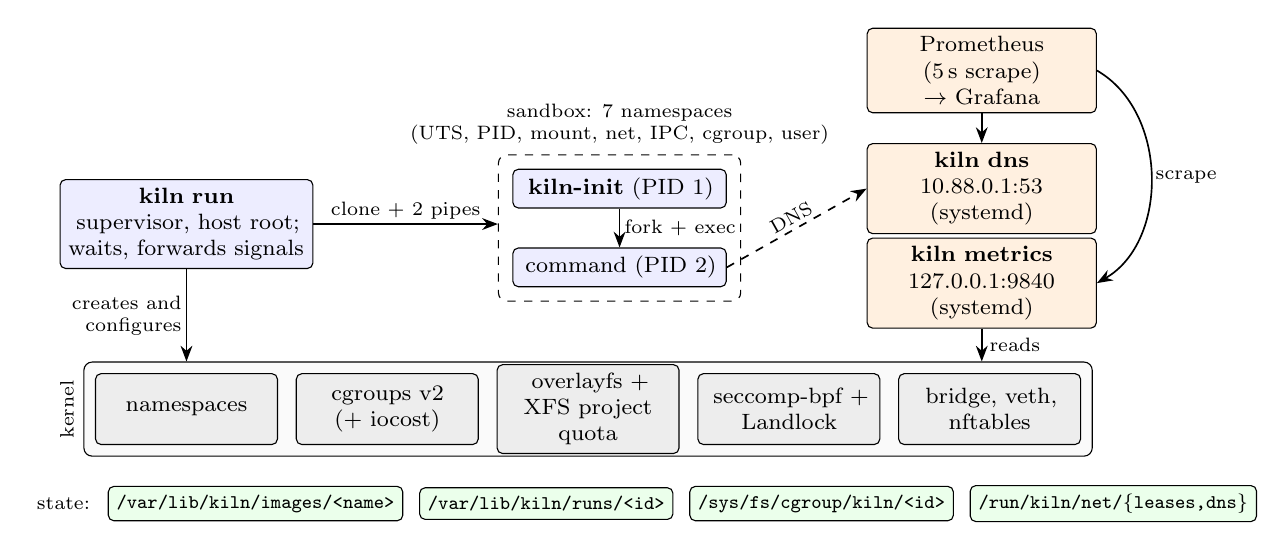
\begin{tikzpicture}[font=\footnotesize]
  % user-space processes
  \node[proc, text width=30mm] (run) at (0,0.1) {\textbf{kiln run}\\supervisor, host root;\\waits, forwards signals};
  \node[proc, text width=25mm] (init) at (5.5,0.55) {\textbf{kiln-init} (PID 1)};
  \node[proc, text width=25mm] (cmd) at (5.5,-0.45) {command (PID 2)};
  \draw[arr] (init) -- node[lab, right] {fork + exec} (cmd);
  \node[draw, dashed, rounded corners=3pt, fit=(init)(cmd), inner sep=5pt,
        label={[font=\scriptsize, align=center]above:sandbox: 7 namespaces\\(UTS, PID, mount, net, IPC, cgroup, user)}] (sb) {};
  \node[svc, text width=27mm] (dns) at (10.1,0.55) {\textbf{kiln dns}\\10.88.0.1:53 (systemd)};
  \node[svc, text width=27mm] (met) at (10.1,-0.65) {\textbf{kiln metrics}\\127.0.0.1:9840 (systemd)};
  \node[svc, text width=27mm] (prom) at (10.1,2.05) {Prometheus (5\,s scrape)\\$\rightarrow$ Grafana};
  \draw[arr] (run) -- node[lab, above] {clone + 2 pipes} (sb.west |- run);
  \draw[arr, dashed] (cmd.east) -- node[lab, above, sloped] {DNS} (dns.west);
  \draw[arr] (prom) -- (dns);
  \draw[arr] (prom.east) to[out=-30, in=30] node[lab, right] {scrape} (met.east);
  % kernel
  \foreach \x/\n/\t in {0/k1/{namespaces},2.55/k2/{cgroups v2\\(+ iocost)},5.1/k3/{overlayfs +\\XFS project quota},7.65/k4/{seccomp-bpf +\\Landlock},10.2/k5/{bridge, veth,\\nftables}}
    \node[kern, text width=21mm, minimum height=9mm] (\n) at (\x,-2.25) {\t};
  \begin{scope}[on background layer]
    \node[draw, fill=gray!4, rounded corners=3pt, fit=(k1)(k5), inner sep=4pt,
          label={[font=\scriptsize]left:\rotatebox{90}{kernel}}] (kern) {};
  \end{scope}
  \draw[arr] (run.south) -- node[lab, left, align=right] {creates and\\configures} (run.south |- kern.north);
  \draw[arr] (met.south) -- node[lab, right, xshift=1pt] {reads} (met.south |- kern.north);
  % state
  \node[st, anchor=west] (s1) at (-1.0,-3.45) {/var/lib/kiln/images/<name>};
  \node[st, right=2mm of s1] (s2) {/var/lib/kiln/runs/<id>};
  \node[st, right=2mm of s2] (s3) {/sys/fs/cgroup/kiln/<id>};
  \node[st, right=2mm of s3] (s4) {/run/kiln/net/\{leases,dns\}};
  \node[font=\scriptsize, left=1mm of s1] {state:};
\end{tikzpicture}
\caption{kiln's parts. The supervisor creates each sandbox and configures the
kernel on its behalf; the two services run under systemd and are shared by all
sandboxes. All state is kernel objects plus the four directories at the bottom.}
\label{fig:arch}
\end{figure}

\textbf{No central manager daemon, no database.} A run's identity is its \emph{run ID}, the start
time in nanoseconds (hex) plus kiln's PID: unique, sortable, and used to name both
its cgroup (\code{/sys/fs/cgroup/kiln/<id>}) and its run directory
(\code{/var/lib/kiln/runs/<id>}). IP leases and DNS policies are files named
after the sandbox's IP, and tools find running sandboxes by listing
\code{/sys/fs/cgroup/kiln/}. The cost of this design is that recovery after a crash
must be explicit: \code{kiln gc} and lease reconciliation (\S\ref{sec:persistent},
\S\ref{sec:net}) rebuild their view from these same files.

\textbf{Resource ownership through RAII.} The supervisor holds a \code{Cgroup}
value and an optional \code{Network} value whose destructors run on every exit
path: the nftables policy and the lease, then \code{cgroup.kill} and
\code{rmdir}, then the run directory (unless \code{--keep}). The overlay mount
and the veth live in the sandbox's namespaces and disappear with them.

% ---------------------------------------------------------------------------
\section{Process and namespace setup}
\label{sec:startup}

A namespace gives a process its own instance of one kind of global kernel
resource. kiln creates five at \code{clone3} time: UTS (hostname), PID (the child
becomes PID 1 of a new numbering), mount, network, and IPC (System V shared
memory, semaphores and message queues). The child later unshares two more: a
cgroup namespace and, last of all, a user namespace. Without \code{CLONE\us{}VM}, \code{clone3} behaves like \code{fork}: the child gets a copy-on-write copy of the parent's memory, configuration included.

\begin{figure}[t]
\centering
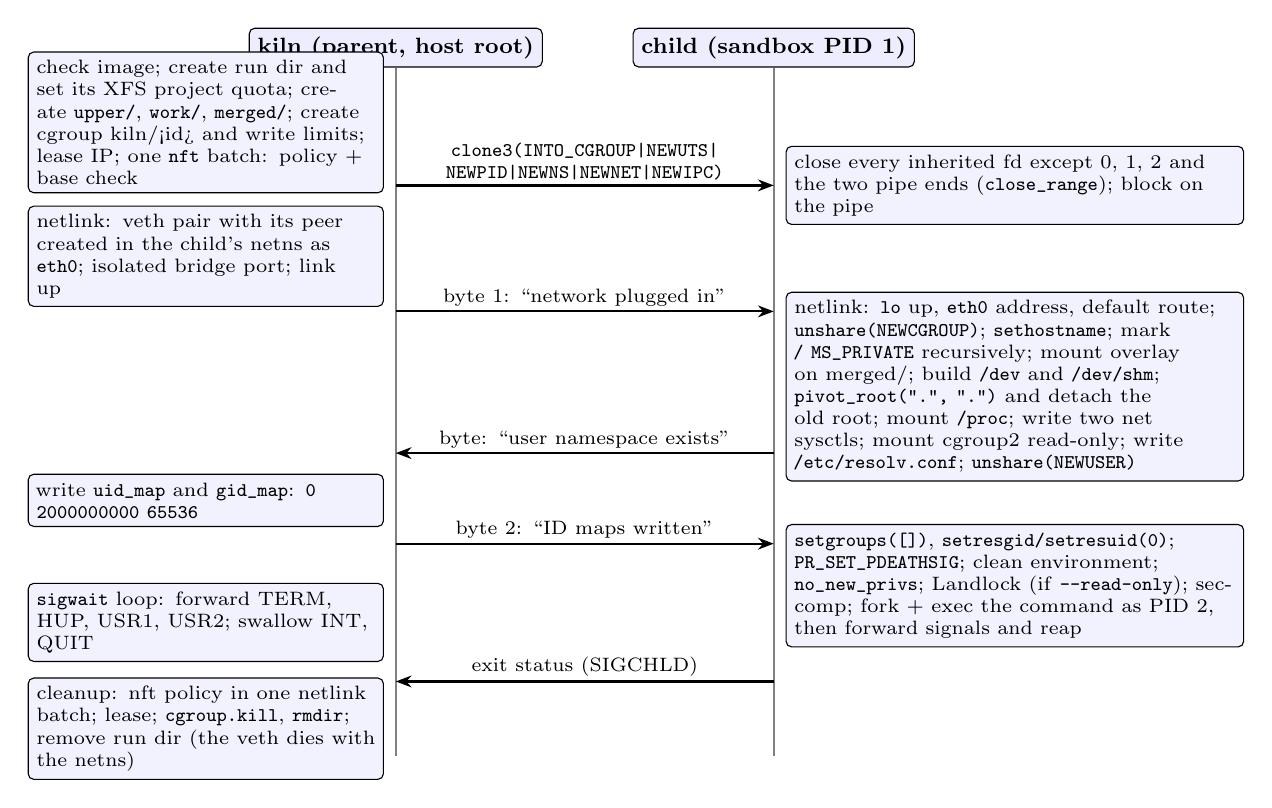
\begin{tikzpicture}[font=\footnotesize,
    pnote/.style={box, fill=blue!5, text width=43mm, align=left, anchor=east, font=\scriptsize},
    cnote/.style={box, fill=blue!5, text width=56mm, align=left, anchor=west, font=\scriptsize},
    msg/.style={arr, thick}]
  \def\P{4.6} \def\C{9.4}
  \node[proc, font=\footnotesize\bfseries] (ph) at (\P,0) {kiln (parent, host root)};
  \node[proc, font=\footnotesize\bfseries] (ch) at (\C,0) {child (sandbox PID 1)};
  \draw[gray, thick] (ph.south) -- (\P,-9.0);
  \draw[gray, thick] (ch.south) -- (\C,-9.0);
  % parent steps
  \node[pnote] at (\P-0.15,-0.95) {check image; create run dir and set its XFS project quota; create \code{upper/}, \code{work/}, \code{merged/}; create cgroup kiln/<id> and write limits; lease IP; one \code{nft} batch: policy + base check};
  \draw[msg] (\P,-1.75) -- node[lab, above, align=center] {\code{clone3(INTO\us{}CGROUP|NEWUTS|}\\\code{NEWPID|NEWNS|NEWNET|NEWIPC)}} (\C,-1.75);
  \node[cnote] at (\C+0.15,-1.75) {close every inherited fd except 0, 1, 2 and the two pipe ends (\code{close\us{}range}); block on the pipe};
  \node[pnote] at (\P-0.15,-2.65) {netlink: veth pair with its peer created in the child's netns as \code{eth0}; isolated bridge port; link up};
  \draw[msg] (\P,-3.35) -- node[lab, above] {byte 1: ``network plugged in''} (\C,-3.35);
  \node[cnote, anchor=north west] at (\C+0.15,-3.1) {netlink: \code{lo} up, \code{eth0} address, default route; \code{unshare(NEWCGROUP)}; \code{sethostname}; mark \code{/} \code{MS\us{}PRIVATE} recursively; mount overlay on merged/; build \code{/dev} and \code{/dev/shm}; \code{pivot\us{}root(".", ".")} and detach the old root; mount \code{/proc}; write two net sysctls; mount cgroup2 read-only; write \code{/etc/resolv.conf}; \code{unshare(NEWUSER)}};
  \draw[msg] (\C,-5.15) -- node[lab, above] {byte: ``user namespace exists''} (\P,-5.15);
  \node[pnote] at (\P-0.15,-5.75) {write \code{uid\us{}map} and \code{gid\us{}map}: \code{0 2000000000 65536}};
  \draw[msg] (\P,-6.3) -- node[lab, above] {byte 2: ``ID maps written''} (\C,-6.3);
  \node[cnote, anchor=north west] at (\C+0.15,-6.05) {\code{setgroups([])}, \code{setresgid/setresuid(0)}; \code{PR\us{}SET\us{}PDEATHSIG}; clean environment; \code{no\us{}new\us{}privs}; Landlock (if \code{--read-only}); seccomp; fork + exec the command as PID~2, then forward signals and reap};
  \node[pnote] at (\P-0.15,-7.3) {\code{sigwait} loop: forward TERM, HUP, USR1, USR2; swallow INT, QUIT};
  \draw[msg] (\C,-8.05) -- node[lab, above] {exit status (SIGCHLD)} (\P,-8.05);
  \node[pnote] at (\P-0.15,-8.65) {cleanup: nft policy in one netlink batch; lease; \code{cgroup.kill}, \code{rmdir}; remove run dir (the veth dies with the netns)};
\end{tikzpicture}
\caption{Sandbox startup. The child is born inside its cgroup; three one-byte
messages over two \code{O\us{}CLOEXEC} pipes order the steps that must happen
outside the sandbox (network plumbing, ID maps) relative to those inside it.
If either side dies, the other reads EOF instead of hanging.}
\label{fig:startup}
\end{figure}

Figure~\ref{fig:startup} is the whole startup protocol. Three ordering
constraints shape it:

\begin{enumerate}
\item \textbf{Limits before the first instruction.} \code{clone3} with
\code{CLONE\us{}INTO\us{}CGROUP} and an open fd of the cgroup directory creates the
child already inside it, so no instruction runs outside its limits. (The older
way, writing the PID to \code{cgroup.procs} before releasing the child, was the
slowest step of a start; \S\ref{sec:perf}.) The network is plugged in before the
child is released.
\item \textbf{The cgroup namespace inside the cgroup.} A cgroup namespace makes
the process's \emph{current} cgroup appear as the root. \code{clone3} creates
namespaces before placing the child, so the child unshares it itself; otherwise
the host's cgroup would become the sandbox's root.
\item \textbf{The user namespace last.} Every namespace is owned by the user
namespace that was current when it was created, and capabilities only act on
namespaces that one's user namespace owns. Creating the user namespace after all
the others leaves them owned by the host, so sandbox root, with a full capability
set, cannot mount, unmount, change the hostname or reconfigure its network.
\end{enumerate}

\textbf{File descriptors are the first thing closed.} Namespaces,
\code{pivot\us{}root} and Landlock all check \emph{paths} at open time; none of
them revokes a descriptor that is already open. A descriptor inherited from
whatever started kiln is therefore a handle straight through every wall
(\S\ref{sec:review}). The child closes everything except stdio and its two pipe
ends before doing anything else, which also means a parent that dies mid-setup
shows up as EOF on the pipe.

% ---------------------------------------------------------------------------
\section{Root filesystem: overlayfs and pivot\_root}

\begin{figure}[t]
\centering
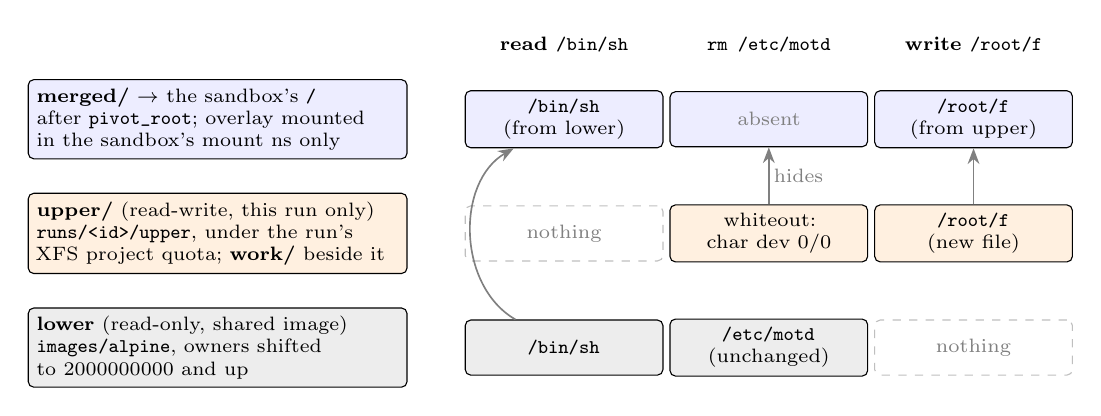
\begin{tikzpicture}[font=\footnotesize,
    layer/.style={box, text width=46mm, align=left, minimum height=10mm, font=\scriptsize},
    cell/.style={box, text width=23mm, minimum height=7mm, font=\scriptsize},
    empty/.style={cell, draw=gray!50, dashed, text=gray}]
  \node[layer, fill=blue!7] (m) at (0,0) {\textbf{merged/} $\rightarrow$ the sandbox's \code{/}\\after \code{pivot\us{}root}; overlay mounted\\in the sandbox's mount ns only};
  \node[layer, fill=orange!12] (u) at (0,-1.45) {\textbf{upper/} (read-write, this run only)\\\code{runs/<id>/upper}, under the run's\\XFS project quota; \textbf{work/} beside it};
  \node[layer, fill=gray!14] (l) at (0,-2.9) {\textbf{lower} (read-only, shared image)\\\code{images/alpine}, owners shifted\\to 2000000000 and up};
  % columns
  \def\a{4.4} \def\b{7.0} \def\c{9.6}
  \node[font=\scriptsize\bfseries] at (\a,0.95) {read \code{/bin/sh}};
  \node[font=\scriptsize\bfseries] at (\b,0.95) {\code{rm /etc/motd}};
  \node[font=\scriptsize\bfseries] at (\c,0.95) {write \code{/root/f}};
  \node[cell, fill=blue!7] (m1) at (\a,0) {\code{/bin/sh}\\(from lower)};
  \node[cell, fill=blue!7, text=gray] (m2) at (\b,0) {absent};
  \node[cell, fill=blue!7] (m3) at (\c,0) {\code{/root/f}\\(from upper)};
  \node[empty] (u1) at (\a,-1.45) {nothing};
  \node[cell, fill=orange!12] (u2) at (\b,-1.45) {whiteout:\\char dev 0/0};
  \node[cell, fill=orange!12] (u3) at (\c,-1.45) {\code{/root/f}\\(new file)};
  \node[cell, fill=gray!14] (l1) at (\a,-2.9) {\code{/bin/sh}};
  \node[cell, fill=gray!14] (l2) at (\b,-2.9) {\code{/etc/motd}\\(unchanged)};
  \node[empty] (l3) at (\c,-2.9) {nothing};
  \draw[arr, gray] (l1) to[out=150, in=-150] (m1);
  \draw[arr, gray] (u2) -- node[lab, right] {hides} (m2);
  \draw[arr, gray] (u3) -- (m3);
\end{tikzpicture}
\caption{The overlay root. Reads fall through to the shared image; writes and
deletions land only in the run's upper layer, so \code{upper/} is an exact record
of what the sandbox changed. On top of \code{merged/}, the sandbox mounts its own
\code{/proc}, a minimal \code{/dev} tmpfs, a 64\,MiB \code{/dev/shm} and a
read-only cgroup2 at \code{/sys/fs/cgroup}.}
\label{fig:overlay}
\end{figure}

Every sandbox shares one read-only image and gets a private writable layer
(Figure~\ref{fig:overlay}). overlayfs merges them: lookups check the upper
layer first; the first write to a lower file copies it up; a deletion leaves a
\emph{whiteout} (a 0/0 character device) in the upper layer. Two consequences
matter for agents. Destroying the image from inside is impossible (\code{rm -rf
/bin} only writes whiteouts), and \code{upper/} is a precise, free audit log of
the run's changes; \code{--keep} preserves it for inspection. Mount points that
kiln itself needs (\code{/sys/fs/cgroup}, \code{/workspace}) are created in the
image at fetch time, so \code{upper/} holds only what the sandbox wrote.

\textbf{Swapping roots.} \code{chroot} only changes how paths are resolved and
leaves the old root reachable to a sufficiently privileged process.
\code{pivot\us{}root} changes the mount namespace's root mount itself. kiln uses
the \code{pivot\us{}root(".", ".")} idiom: with the current directory at the new
root, the old root ends up stacked on top of it, and \code{umount2(".",
MNT\us{}DETACH)} then removes it, leaving no mount through which the host
filesystem can be reached.

\textbf{Mount propagation.} On systemd hosts \code{/} is a \emph{shared} mount, so
even in a new mount namespace, new mounts would propagate back to the host, and
\code{pivot\us{}root} refuses to operate on shared mounts. The child first marks
everything \code{MS\us{}REC|MS\us{}PRIVATE}. During a run, \code{findmnt -t
overlay} on the host is empty.

\textbf{A minimal /dev.} Instead of the host's \code{/dev} (which includes disks),
the sandbox gets a 64\,KiB tmpfs holding bind mounts of six devices (\code{null},
\code{zero}, \code{full}, \code{random}, \code{urandom}, \code{tty}), the usual
\code{fd} and \code{std*} symlinks, and a \code{/dev/shm} tmpfs whose pages are
charged to the sandbox's memory limit. A fresh \code{/proc} (mounted
\code{nosuid,nodev,noexec}) shows only the sandbox's PID namespace.

% ---------------------------------------------------------------------------
\section{Resource limits with cgroups v2}

cgroup v2 is a single hierarchy of directories; each directory is a group of
processes, and controller files inside it set limits and report usage. Two rules
shape kiln's layout (Figure~\ref{fig:cgroups}). Controllers are enabled
top-down: a cgroup can only use \code{memory}, \code{cpu}, \code{pids} or
\code{io} if its parent lists them in \code{cgroup.subtree\us{}control}. And a
cgroup that delegates controllers to children cannot hold processes itself (``no
internal processes''). So sandboxes live \emph{under} \code{/sys/fs/cgroup/kiln/},
which itself stays empty.

\begin{figure}[t]
\centering
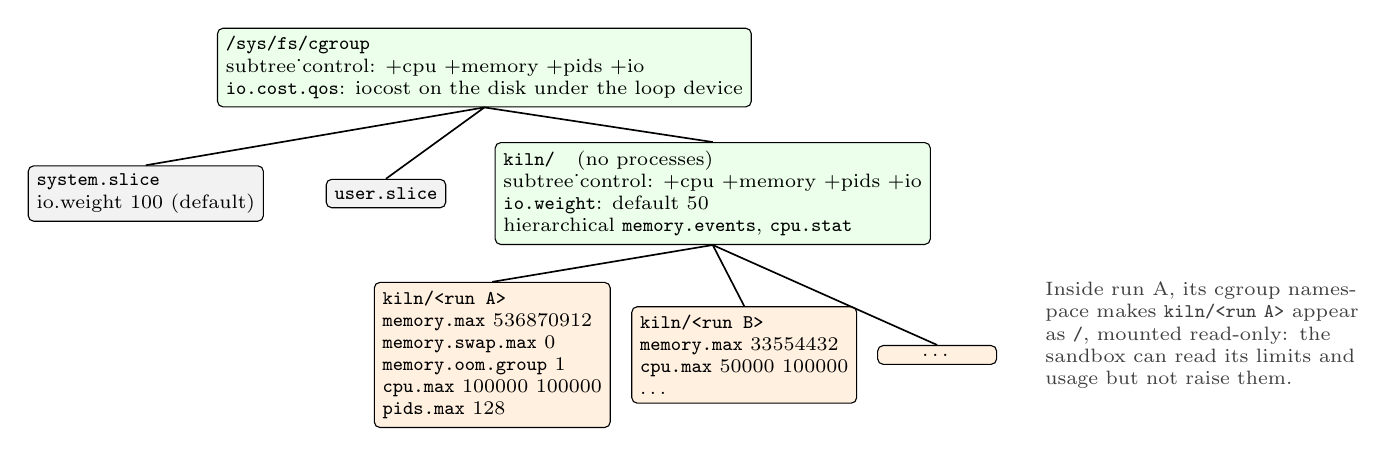
\begin{tikzpicture}[font=\scriptsize,
    cg/.style={box, fill=green!8, font=\scriptsize, align=left},
    note/.style={font=\scriptsize, align=left, text=black!75}]
  \node[cg] (root) at (0,0) {\code{/sys/fs/cgroup}\\subtree\us{}control: +cpu +memory +pids +io\\\code{io.cost.qos}: iocost on the disk under the loop device};
  \node[cg, fill=gray!10] (sys) at (-4.3,-1.6) {\code{system.slice}\\io.weight 100 (default)};
  \node[cg, fill=gray!10] (usr) at (-1.25,-1.6) {\code{user.slice}};
  \node[cg] (kiln) at (2.9,-1.6) {\code{kiln/}\quad (no processes)\\subtree\us{}control: +cpu +memory +pids +io\\\code{io.weight}: default 50\\hierarchical \code{memory.events}, \code{cpu.stat}};
  \node[cg, fill=orange!12] (a) at (0.1,-3.65) {\code{kiln/<run A>}\\\code{memory.max} 536870912\\\code{memory.swap.max} 0\\\code{memory.oom.group} 1\\\code{cpu.max} 100000 100000\\\code{pids.max} 128};
  \node[cg, fill=orange!12] (b) at (3.3,-3.65) {\code{kiln/<run B>}\\\code{memory.max} 33554432\\\code{cpu.max} 50000 100000\\\ldots};
  \node[cg, fill=orange!12, text width=13mm, align=center] (c) at (5.75,-3.65) {\ldots};
  \foreach \n in {sys,usr,kiln} \draw[semithick] (root.south) -- (\n.north);
  \foreach \n in {a,b,c} \draw[semithick] (kiln.south) -- (\n.north);
  \node[note, anchor=west, text width=40mm] at (7.0,-3.4) {Inside run A, its cgroup namespace makes \code{kiln/<run A>} appear as \code{/}, mounted read-only: the sandbox can read its limits and usage but not raise them.};
\end{tikzpicture}
\caption{cgroup hierarchy. Limits are set per run; the parent sets the sandboxes'
collective I/O share and provides counters that survive individual runs.}
\label{fig:cgroups}
\end{figure}

\begin{table}[t]
\centering\small
\caption{Limits, their defaults, and the kernel interface behind each.}
\label{tab:limits}
\begin{tabularx}{\linewidth}{@{}l l >{\raggedright\arraybackslash}X >{\raggedright\arraybackslash}X@{}}
\toprule
Flag & Default & Kernel interface & At the limit \\
\midrule
\code{--memory} & 512M & \code{memory.max}; \code{memory.swap.max}=0; \code{memory.oom.group}=1 & reclaim, then the OOM killer kills every process in the sandbox \\
\code{--cpus} & 1 & \code{cpu.max} = ``$q$ 100000'', $q$ = cores $\times$ 100\,000\,\textmu s & throttled for the rest of each 100\,ms period \\
\code{--pids} & 128 & \code{pids.max} & \code{fork}/\code{clone} fail; counted in \code{pids.events} \\
\code{--disk} & 1G & XFS project quota: block hard limit, plus one inode per 16\,KiB (min.\ 128) & writes fail with \code{ENOSPC} \\
(all runs) & --- & parent \code{io.weight} ``default 50'' with iocost & proportional share, only under contention \\
(all runs) & --- & tmpfs \code{size=}: 64\,KiB \code{/dev}, 64\,MiB \code{/dev/shm} & \code{ENOSPC}; shm pages count toward \code{memory.max} \\
\bottomrule
\end{tabularx}
\end{table}

Table~\ref{tab:limits} lists every limit. The design decisions behind them:

\begin{itemize}
\item \textbf{Kill the sandbox, not a process.} \code{memory.oom.group} makes an
OOM kill take out the whole group. A half-killed tool call (a shell whose child
died) is harder to reason about than one that failed outright. Swap is disabled
for the group (when a memory limit is set) so a memory hog hits its limit instead of degrading into swap.
\item \textbf{CPU is a quota per period}, not a share: \code{--cpus 0.25} writes
\code{25000 100000}, so a 2\,s busy loop gets 500\,ms of CPU.
\item \textbf{Page cache is memory.} Writing 100\,MB showed a memory peak of
about 100\,MiB: file pages are charged to the writer's cgroup. They are
reclaimable, but they count toward \code{memory.max} (\S\ref{sec:io}).
\item \textbf{Teardown is atomic.} \code{cgroup.kill} SIGKILLs every process in
the group in one write, including anything that left the command's process tree.
\end{itemize}

% ---------------------------------------------------------------------------
\section{kiln-init: PID 1 and signals}

The kernel treats a PID namespace's init specially: signals sent to it from
inside its namespace are dropped unless it installed a handler, and orphaned
processes are re-parented to it. A normal program as PID 1 therefore ignores
\code{kill} and \code{timeout} and never reaps orphans. Before kiln-init,
\code{kiln run -- timeout 2 sh -c 'while :; do :; done'} never ended: busybox
\code{timeout} signalled from inside the namespace and PID 1 ignored it.

So PID 1 is kiln itself (the same binary, already running in the child), playing
the role \code{tini} plays for Docker. It blocks all signals, forks the command
as PID 2 (which restores an empty mask and \code{exec}s), and then loops on
\code{sigwait}: on SIGCHLD it reaps \emph{every} exited child (several exits can
coalesce into one signal), and SIGTERM, SIGHUP, SIGUSR1 and SIGUSR2 are forwarded
to the command. When the command exits, init returns its status (128 + signal
number if it was killed, 127 if \code{exec} failed) and exits; the kernel then
kills whatever is left in the PID namespace.

\textbf{Waiting for signals rather than handling them.} Both kiln-init and the
supervisor block signals with \code{sigprocmask} and consume them synchronously
with \code{sigwait} in the same loop that reaps children. There are no
asynchronous handlers, so there are no async-signal-safety rules to get wrong.
The supervisor therefore survives Ctrl-C and \code{kill} and still cleans up.
SIGINT, SIGQUIT and SIGWINCH are not forwarded: the terminal already sends them
to its whole foreground process group, which includes the sandboxed command.

% ---------------------------------------------------------------------------
\section{Persistent sandboxes}
\label{sec:persistent}

Agents need state between tool calls: a package installed by one command must
be there for the next. \code{kiln create} starts a sandbox that outlives the
command that created it and prints its ID; \code{kiln exec <id> -- <cmd>} runs a
command in it; \code{kiln ls} lists sandboxes and whether their shim is alive;
\code{kiln rm} stops one and waits until its resources are gone; and \code{kiln
gc} cleans up after shims that died. One-shot \code{kiln run} is unchanged.

\begin{figure}[t]
\centering
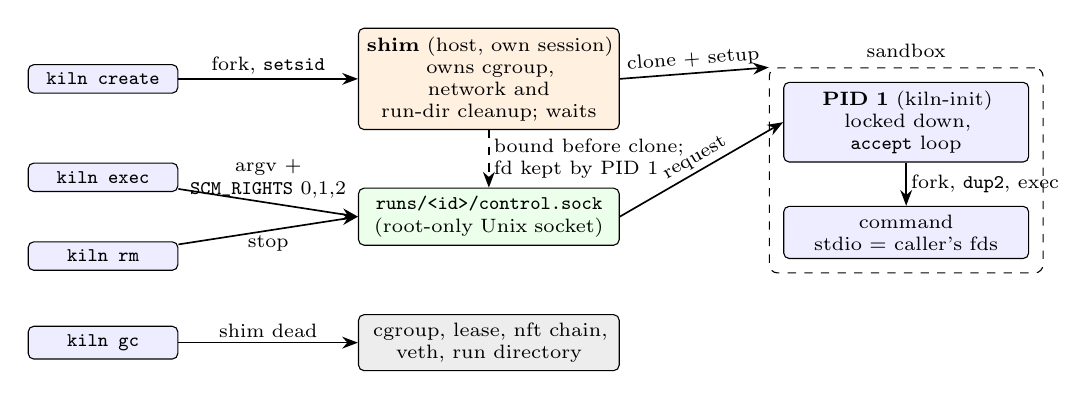
\begin{tikzpicture}[font=\scriptsize,
    cli/.style={box, fill=blue!7, font=\scriptsize\ttfamily, minimum width=19mm},
    note/.style={font=\scriptsize, align=left}]
  \node[cli] (create) at (0,1.5) {kiln create};
  \node[cli] (exec) at (0,0.25) {kiln exec};
  \node[cli] (rm) at (0,-0.75) {kiln rm};
  \node[cli] (gc) at (0,-1.85) {kiln gc};
  \node[svc, text width=31mm] (shim) at (4.9,1.5) {\textbf{shim} (host, own session)\\owns cgroup, network and\\run-dir cleanup; waits};
  \node[st, text width=31mm, align=center] (sock) at (4.9,-0.25) {runs/<id>/control.sock\\\normalfont(root-only Unix socket)};
  \node[kern, text width=31mm, font=\scriptsize] (left) at (4.9,-1.85) {cgroup, lease, nft chain,\\veth, run directory};
  \node[proc, text width=29mm] (init) at (10.2,0.95) {\textbf{PID 1} (kiln-init)\\locked down, \code{accept} loop};
  \node[proc, text width=29mm] (cmd) at (10.2,-0.45) {command\\stdio = caller's fds};
  \node[draw, dashed, rounded corners=3pt, fit=(init)(cmd), inner sep=5pt,
        label={[font=\scriptsize]above:sandbox}] (sb) {};
  \draw[arr] (create) -- node[lab, above] {fork, \code{setsid}} (shim);
  \draw[arr] (shim.east) -- node[lab, above, sloped] {clone + setup} (sb.north west);
  \draw[arr, dashed] (shim) -- node[lab, right, align=left] {bound before clone;\\fd kept by PID 1} (sock);
  \draw[arr] (exec) -- node[lab, above, align=center] {argv +\\\code{SCM\us{}RIGHTS} 0,1,2} (sock.west);
  \draw[arr] (rm) -- node[lab, below] {stop} (sock.west);
  \draw[arr] (sock.east) -- node[lab, above, sloped] {request} (init.west);
  \draw[arr] (init) -- node[lab, right] {fork, \code{dup2}, exec} (cmd);
  \draw[arr] (gc) -- node[lab, above] {shim dead} (left);
\end{tikzpicture}
\caption{Persistent sandboxes. A detached shim owns each sandbox's host
resources; PID 1 serves \code{exec} and \code{rm} requests on a socket opened
before \code{pivot\us{}root}. Exit codes travel back over the same connection.
\code{kiln gc} removes what a dead shim left behind.}
\label{fig:persistent}
\end{figure}

\textbf{A shim per sandbox.} \code{kiln create} forks a host process, which
starts its own session, detaches from the terminal, and does exactly what the
one-shot supervisor does (run directory and quota, cgroup, \code{clone},
network, ID maps), then reports ready over a pipe so the CLI can print the ID
and exit. The shim stays alive as the sandbox's parent, holding the
\code{Cgroup} and \code{Network} values whose destructors clean up. This is
containerd's shim pattern: a sandbox's lifetime is tied to a small process
dedicated to it, not to the CLI or a future daemon. If the shim is killed,
\code{PR\us{}SET\us{}PDEATHSIG} takes PID 1 down, and \code{kiln gc} finds run
directories whose shim is dead and removes their cgroup, network state and files
(Figure~\ref{fig:persistent}).

\textbf{Exec through PID 1, not \code{setns}.} The usual design is for the host
to enter the sandbox's namespaces with \code{setns}, as \code{docker exec} does
through runc. A process entering from outside arrives without the sandbox's
credentials, cgroup, Landlock ruleset or seccomp filter, and each must be
re-applied in the right order: a second code path for every ordering constraint
of \S\ref{sec:startup}. kiln makes the sandbox's own PID 1 the exec server
instead. Before cloning, the shim binds a Unix socket in the run directory. The
child keeps that one descriptor when it closes all others, completes the full
lockdown, sends a third handshake byte, and loops on \code{accept}. \code{kiln
exec} connects, sends the argument vector as a length-prefixed message, and
passes redirected stdin, stdout and stderr as \code{SCM\us{}RIGHTS} descriptors.
It refuses terminal descriptors until kiln has a controlled PTY mode. PID 1
forks, duplicates them onto 0--2, and \code{exec}s: the command inherits every
namespace, limit, filter and rule simply by being PID 1's child. PID 1 reaps it
and writes the exit status back, so \code{kiln exec} exits with the command's
own code.

\textbf{Consequences.} After lockdown, the only host objects the sandbox can
reach are the listening socket (whose path is not visible inside) and the
descriptors a caller chose to pass. Requests are size-bounded and parsed
strictly, and run one at a time. Files persist in the upper layer. Running
\code{true} this way takes 3.5\,ms (p50, one client, uncontended), against 9.7
to 53.7\,ms for the other runtimes' \code{exec} (\S\ref{sec:perf}). \code{kiln rm} sends a stop request; PID 1 acknowledges and exits, the
kernel kills the rest of the PID namespace, and the shim's normal cleanup runs.

% ---------------------------------------------------------------------------
\section{Disk quotas with XFS project quotas}

Without a disk limit, one sandbox can fill the host filesystem. Classic quotas
limit what a UID owns, which does not fit (all sandboxes map to the same host IDs,
\S\ref{sec:userns}). XFS \emph{project} quotas instead limit whatever is tagged
with a 32-bit project ID, and the \code{PROJINHERIT} flag on a directory makes
everything created beneath it inherit the tag. This is how Docker's overlay2 driver
limits container size.

\textbf{Storage.} \code{/var/lib/kiln/runs} is an XFS filesystem inside a sparse
file (20\,GB by default), mounted through a loop device with \code{prjquota}, so no spare
partition is needed. Per run, kiln tags the still-empty run directory with
\code{FS\us{}IOC\us{}FSSETXATTR} (project ID plus \code{PROJINHERIT}) and sets the
limits with \code{quotactl\us{}fd} (\code{Q\us{}XSETQLIM}), both as raw
\code{ioctl}/syscall calls against \code{\#[repr(C)]} structs whose sizes are
asserted at compile time. \code{upper/} and \code{work/} are created afterwards,
so they and everything the sandbox writes are charged to the run.

\textbf{Design decisions.} (1)~The project ID is the run directory's inode
number: unique on the filesystem for as long as the directory exists, so no ID
allocator is needed. (2)~Because inode numbers are reused, kiln \emph{always}
writes the limit, even ``unlimited'' (0); otherwise a new run could inherit a
dead run's limit. (3)~Blocks alone are not enough: empty files cost almost no
blocks, so a small block quota could still exhaust the filesystem's inodes. Each
project also gets an inode limit of one per 16\,KiB of quota (at least 128).
(4)~A full quota surfaces to the program as \code{ENOSPC} (``No space left on
device''), not \code{EDQUOT}, which is the honest description from inside.

% ---------------------------------------------------------------------------
\section{User namespaces and ID mapping}
\label{sec:userns}

Without a user namespace, root in the sandbox is root on the host, and every
other wall becomes the last one. With it, sandbox UIDs and GIDs 0--65535 map to
host IDs 2\,000\,000\,000--2\,000\,065\,535, a range no real user owns (well above
the \code{/etc/subuid} range given to the VM's user). An escaped process lands on
the host as UID 2\,000\,000\,000, which owns nothing.

\textbf{Only an outsider can write the maps.} A fresh user namespace has no
mapping, so its process appears as the overflow ID (\code{nobody}). The parent,
which holds \code{CAP\us{}SETUID}/\code{CAP\us{}SETGID} over the parent namespace,
writes \code{0 2000000000 65536} to the child's \code{uid\us{}map} and
\code{gid\us{}map}; the child then drops supplementary groups and switches to
UID/GID 0. That is the second pipe handshake in Figure~\ref{fig:startup}.

\textbf{Capabilities that apply to nothing.} Inside, root has a full capability
set (\code{CapEff: 000001ffffffffff}), but since the mount, UTS, network, IPC,
PID and cgroup namespaces are owned by the host's user namespace,
\code{hostname}, \code{mount}, \code{umount} and \code{ip link set} all fail with
\code{EPERM}.

\textbf{Image files must be shifted.} Host-root-owned image files would appear as
\code{nobody} inside, and sandbox root could not modify them. The fetch script
therefore adds 2\,000\,000\,000 to every file's owner and group, restoring setuid
bits that \code{chown} clears (Docker's userns-remap approach), and kiln refuses
to start if the image root is not owned by the base ID. The upper layer is
chowned to the same ID so the sandbox's \code{/} belongs to sandbox root. The
known cost is that all sandboxes share one ID range (\S\ref{sec:limits}).

\textbf{Trusting the image.} The image is the root filesystem of every sandbox,
so the fetch script treats the download as hostile until proven otherwise. It
accepts only a strictly formed \code{alpine-minirootfs-*-<arch>.tar.gz} name,
checks the published SHA-256, and verifies the detached signature with
\code{gpgv} against Alpine's release key, which is pinned in the repository by
fingerprint. A checksum from the same server as the file proves only integrity;
the signature proves who published it. The image is then unpacked and shifted in
a staging directory on the same filesystem and swapped in with
\code{renameat2(RENAME\us{}EXCHANGE)}, so a sandbox starting during an update
sees either the old image or the new one, never a half-written tree.

Because sandbox root does not own its network namespace, it could not bind
ports below 1024 or ping; the child sets two per-namespace sysctls
(\code{ip\us{}unprivileged\us{}port\us{}start}, \code{ping\us{}group\us{}range}) to
allow both, as Docker does.

% ---------------------------------------------------------------------------
\section{Syscall filtering and Landlock}

Namespaces control what a process can \emph{see}; the kernel is still shared, and
every system call is attack surface. Two final restrictions are applied just
before the command starts, both inherited by every descendant and irrevocable.

\textbf{no\_new\_privs} comes first. It guarantees that \code{exec} can never grant
more privilege (setuid bits stop working), which is the precondition for an
unprivileged process to install a seccomp filter or Landlock ruleset: otherwise a
filtered process could exec a setuid binary that runs with the filter but with
more privilege.

\textbf{seccomp-bpf.} A seccomp filter is a small classic-BPF program the kernel
runs on every syscall, over a struct holding the architecture, syscall number and
arguments. kiln's is hand-assembled. It first checks the architecture, since
syscall numbers differ per ABI, and kills the process on a mismatch (and, on
x86-64, on x32 syscalls). It then denies, with \code{EPERM}, about 40 syscalls in
a few families: loading kernel modules and kexec; large, historically bug-prone
subsystems (\code{bpf}, \code{perf\us{}event\us{}open}, \code{userfaultfd},
\code{io\us{}uring}); the kernel keyring, which is not namespaced;
open-by-handle, which bypasses path checks; \code{setns} and the whole mount API;
and host-wide state (clocks, swap, accounting, kernel log, quotas). Finally it
denies any \code{clone} or \code{unshare} whose flags include a
\code{CLONE\us{}NEW*} bit. That matters because sandbox root holds every capability
\emph{inside} its user namespace: a new network or mount namespace it created
would be its own, exposing root-only kernel code. \code{clone3} passes its flags
in memory the filter cannot read, so it returns \code{ENOSYS}, which makes libc
fall back to \code{clone} (the approach Docker uses). The filter is installed
with \code{SECCOMP\us{}FILTER\us{}FLAG\us{}TSYNC}, a no-op for today's
single-threaded child but correct for a future multi-threaded one.

\emph{Decision: a denylist}, readable in one sitting, rather than an allowlist
like Docker's ($\sim$350 syscalls); the cost is that new syscalls are allowed.

\textbf{Landlock} (with \code{--read-only}) restricts which paths may be written,
and unlike file permissions it binds root (\code{CAP\us{}DAC\us{}OVERRIDE} does not
apply). A ruleset declares the access rights it \emph{handles}; any handled right
is denied unless a rule grants it beneath some directory. kiln handles only
write-type rights (writing, truncating, creating, removing and renaming across
directories), so reading and executing stay allowed everywhere, and grants them
beneath \code{/tmp}, \code{/root}, \code{/workspace}, \code{/dev/shm} and any
\code{--writable} paths; existing \code{/dev} files stay writable but no new
devices can be created. kiln requires Landlock ABI~3 (Linux 6.2), the first that
covers truncation; on older kernels \code{--read-only} would silently allow files
to be emptied. Landlock does not cover metadata, so \code{chmod} on a file the
sandbox owns still works.

% ---------------------------------------------------------------------------
\section{Networking: bridge, veth pairs and nftables}
\label{sec:net}

Every sandbox gets its own network namespace. With \code{--net none} (the
default) it contains only loopback. With \code{--net full} or \code{--allow}, the
supervisor connects it to the host (Figure~\ref{fig:net}).

\begin{figure}[t]
\centering
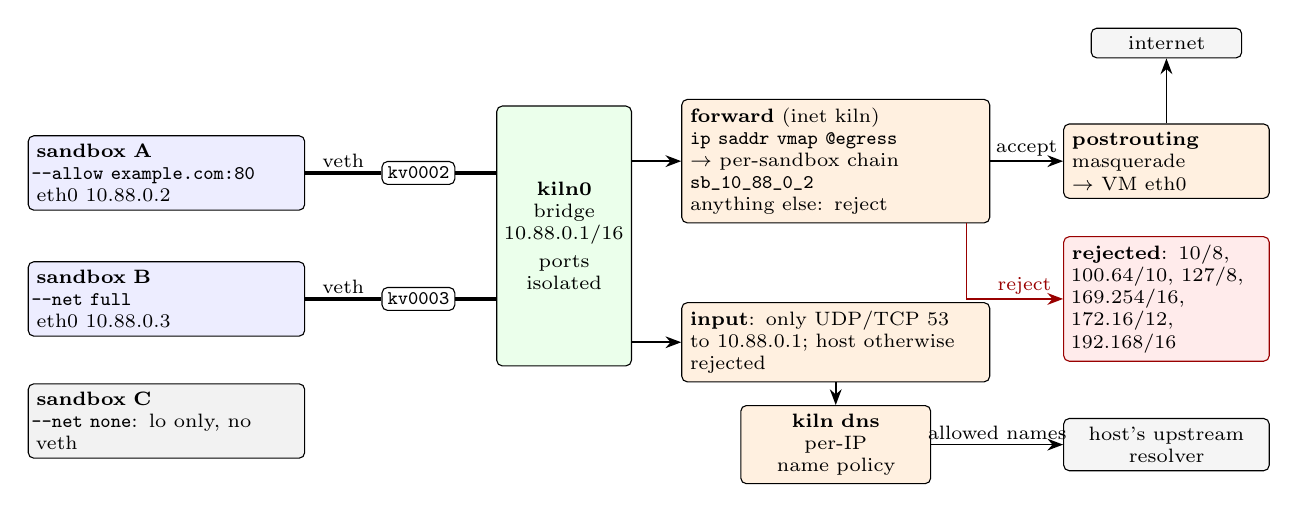
\begin{tikzpicture}[font=\scriptsize,
    ns/.style={box, fill=blue!7, text width=33mm, align=left, font=\scriptsize},
    ifc/.style={box, fill=white, font=\scriptsize\ttfamily, inner sep=2pt},
    rule/.style={box, fill=orange!12, align=left, font=\scriptsize},
    bad/.style={box, fill=red!8, draw=red!60!black, align=left, font=\scriptsize}]
  \node[ns] (a) at (-0.3,1.1) {\textbf{sandbox A}\\\code{--allow example.com:80}\\eth0 10.88.0.2};
  \node[ns] (b) at (-0.3,-0.5) {\textbf{sandbox B}\\\code{--net full}\\eth0 10.88.0.3};
  \node[ns, fill=gray!10] (c) at (-0.3,-2.05) {\textbf{sandbox C}\\\code{--net none}: lo only, no veth};
  \node[ifc] (va) at (2.9,1.1) {kv0002};
  \node[ifc] (vb) at (2.9,-0.5) {kv0003};
  \draw[very thick] (a.east) -- node[lab, above] {veth} (va.west);
  \draw[very thick] (b.east) -- node[lab, above] {veth} (vb.west);
  \node[box, fill=green!8, minimum height=33mm, text width=15mm] (br) at (4.75,0.3) {\textbf{kiln0}\\bridge\\10.88.0.1/16\\[2pt]ports\\isolated};
  \draw[very thick] (va.east) -- (va.east -| br.west);
  \draw[very thick] (vb.east) -- (vb.east -| br.west);
  \node[rule, text width=37mm] (fwd) at (8.2,1.25) {\textbf{forward} (inet kiln)\\\code{ip saddr vmap @egress}\\$\rightarrow$ per-sandbox chain \code{sb\us{}10\us{}88\us{}0\us{}2}\\anything else: reject};
  \node[rule, text width=37mm] (inp) at (8.2,-1.05) {\textbf{input}: only UDP/TCP 53\\to 10.88.0.1; host otherwise\\rejected};
  \node[svc, text width=22mm] (dns) at (8.2,-2.35) {\textbf{kiln dns}\\per-IP name policy};
  \node[rule, text width=24mm] (nat) at (12.4,1.25) {\textbf{postrouting}\\masquerade\\$\rightarrow$ VM eth0};
  \node[box, fill=gray!8, text width=17mm] (net) at (12.4,2.75) {internet};
  \node[bad, text width=24mm] (priv) at (12.4,-0.5) {\textbf{rejected}: 10/8, 100.64/10, 127/8, 169.254/16, 172.16/12, 192.168/16};
  \node[box, fill=gray!8, text width=24mm] (up) at (12.4,-2.35) {host's upstream\\resolver};
  \draw[arr] (br.east |- fwd) -- (fwd.west);
  \draw[arr] (br.east |- inp) -- (inp.west);
  \draw[arr] (inp) -- (dns);
  \draw[arr] (fwd) -- node[lab, above] {accept} (nat);
  \draw[arr] (nat) -- (net);
  \draw[arr, red!60!black] ($(fwd.south east)+(-0.3,0)$) |- node[lab, pos=0.8, above] {reject} (priv.west);
  \draw[arr] (dns) -- node[lab, above] {allowed names} (up);
\end{tikzpicture}
\caption{Network topology. Each networked sandbox has a veth pair whose host end
is an isolated port on \code{kiln0}. All policy is in one nftables table: a
verdict map sends each sandbox's packets to its own chain, the input chain admits
only DNS to the forwarder, and NAT masquerades the rest out of the VM.}
\label{fig:net}
\end{figure}

\textbf{Plumbing from outside.} The network namespace is created at \code{clone3}
time, before the user namespace, so sandbox root cannot change its address,
routes or firewall. The supervisor leases an address and installs the sandbox's
nftables chain before the clone, then creates a veth pair whose peer is created
directly inside the child's namespace as \code{eth0} and attaches the host end to
\code{kiln0} as an isolated port. kiln-init, still real root and before its user
namespace exists, brings up \code{lo}, assigns its address and adds a default
route via 10.88.0.1. Both sides speak rtnetlink directly (a small hand-written
client), the protocol \code{ip} uses, rather than starting \code{ip} or
\code{nsenter}.

\textbf{Shared state is reconciled, not just detected.} The bridge and the base
nftables objects are shared by all sandboxes, so every networked run checks them
under one \code{flock}. The sandbox's policy batch ends with \code{list table},
and that one listing is compared with the canonical sets, map, counters and hook
chains. Only drift is committed as a repair, in one transaction that leaves
per-sandbox chains alone; a canonical ruleset (every run after the first) commits
nothing.

\textbf{Leases.} A lease is a file in \code{/run/kiln/net/leases} created with
\code{O\us{}EXCL}, so concurrent runs cannot get the same address. A lease left by
a killed supervisor is reclaimed only when \emph{every} sign of its run is gone
(cgroup, veth, nft map entry, live supervisor): any one of them is absent during
part of a healthy setup. Leases on the \code{/run} tmpfs vanish on reboot.

\textbf{Policy is one verdict map.} The base table's forward chain is:
\begin{lstlisting}
iifname "kiln0" ct state new add @connlimit { ip saddr ct count over 256 } \
    counter name "conntrack_rejected" counter reject with icmpx admin-prohibited
iifname "kiln0" ip saddr vmap @egress   # jump to this sandbox's chain
iifname "kiln0" counter reject with icmpx admin-prohibited
oifname "kiln0" ct state established,related accept
oifname "kiln0" counter drop
\end{lstlisting}
Adding a sandbox is one map element plus one chain; removing it deletes both, with
no rule handles to track. For \code{--net full} the chain rejects the private
and link-local set (the VM's LAN, the Mac behind it, cloud metadata at
169.254.169.254) and accepts the rest. For \code{--allow HOST[:PORT]} it accepts
only the listed addresses (hostnames are resolved once, at start) and rejects
everything else. The sandbox's source address is trustworthy because sandbox root
cannot change it. Rules end in \code{reject} rather than \code{drop}, so a blocked
connection fails in milliseconds instead of hanging until a timeout, which matters
for an agent waiting on a tool call.

\textbf{Bounding a host-wide table.} The conntrack table is shared by the whole
host; one sandbox opening many distinct flows could fill it. The first rule
counts tracked connections per source IP in a dynamic set and rejects new flows
beyond 256. Because IPs are reused, the IP's count is destroyed at setup and
teardown (\S\ref{sec:review}).

\textbf{Isolation between sandboxes.} Frames between two ports of one bridge are
switched, not routed, so the inet forward hook never sees them. kiln sets the
bridge port flag \code{isolated on} instead, which stops isolated ports from
talking to each other at layer~2. The input chain keeps sandboxes off the host's
own services (\code{sshd}, and later kilnd's API).

% ---------------------------------------------------------------------------
\section{The DNS forwarder}

Name resolution was the last way out: DNS can carry data in query names
(\code{<secret>.attacker.example}), and originally sandboxes could reach the VM's
resolver directly. Now each networked sandbox's \code{/etc/resolv.conf} (written
as real root, so read-only inside) points at \code{kiln dns} on 10.88.0.1:53, the
only resolver the input chain lets it reach. For each query the forwarder reads
the policy file named after the sender's IP: \code{*} for \code{--net full},
otherwise the \code{--allow} hostnames and their subdomains. Allowed queries go
to the host's upstream resolver; others, and senders with no policy file, get
\code{REFUSED}, so with \code{--allow} an attacker's domain is never resolved.

It parses only what it needs (the 12-byte header with exactly one question, then
length-prefixed labels; compression pointers are rejected), accepts upstream
replies only with a matching transaction ID, and turns upstream failures into
\code{SERVFAIL}. Since sandboxes can send it unlimited traffic, 16 workers serve
a queue of 256 jobs and drop on overflow (clients retry), and the systemd unit
caps tasks and memory. Every query is logged with control characters escaped and
counted for Prometheus. The bounds and the escaping came from the second review
(\S\ref{sec:review}).

% ---------------------------------------------------------------------------
\section{Storage and I/O accounting}
\label{sec:io}

\textbf{An OOM kill caused by someone else's cache.} A sandbox writing 1.5\,GB
with \code{O\us{}DIRECT} under a 512\,MB limit was OOM-killed: the loop driver
wrote the XFS image's backing file through the page cache, and those dirty pages
were charged to the sandbox that caused the I/O. Direct I/O on the loop device
(\code{LOOP\us{}SET\us{}DIRECT\us{}IO}, checked on every run) removed the double
caching; the same test peaked at 2.4\,MiB. \textbf{Proportional I/O.}
\code{io.weight} needs a proportional controller, and the VM's disk uses
\code{mq-deadline} without BFQ, so kiln enables iocost on the real disk under the
loop device and gives all sandboxes together half a host service's weight.
Writes are accounted per sandbox in \code{io.stat}, but on this VM the weights do
not change throughput: iocost enforces them only when its model judges the
device saturated, which the Mac's SSD behind virtio never is under the default
model. Accounting works; enforcement is unproven.

% ---------------------------------------------------------------------------
\section{Metrics: Prometheus and Grafana}

\textbf{A stateless exporter.} \code{kiln metrics} reads the kernel's own
counters on every scrape: each sandbox cgroup's memory, CPU, PIDs, \code{io.stat}
and pressure (PSI) files, its XFS project quota, the host end of its veth, and
\code{nft list table inet kiln}, written in the Prometheus text format by hand.
Prometheus scrapes every 5\,s because most sandboxes live for seconds, and a
provisioned Grafana dashboard shows the result.

\textbf{Short runs fall between scrapes.} A sandbox OOM-killed half a second after
starting never appears in a scrape. The parent's \code{kiln/memory.events} and
\code{kiln/cpu.stat} are hierarchical and keep counting after children are
removed, so totals since boot include every run (though the parent's
\code{nr\us{}throttled} counts only its own limit). Rejected packets likewise also
bump a named nftables counter that outlives per-sandbox chains. Two readings need
care: a veth is a mirror (the sandbox's sent bytes are the host end's received
bytes), and with \code{memory.oom.group}, \code{oom\us{}kill} counts processes,
not sandboxes.

% ---------------------------------------------------------------------------
\section{Startup performance}
\label{sec:perf}

For an agent, a sandbox start sits on the critical path of every tool call, so
start latency was measured and then optimized. \textbf{Method:} the v2 harness
times a one-shot \code{true} from immediately before process spawn until the
CLI's \code{waitpid} returns: runtime setup, the command and synchronous cleanup
through CLI exit, with the image local. Kernel-deferred destruction, such as a
veth tied to a dying namespace, can finish after the timer. Every measured
round contains every runtime in seeded,
randomized Latin-square order. The primary campaign used 10 warm-up and 100
measured rounds at a defined 100\,ms idle gap across five fresh VM boots; a
95\% interval bootstraps the geometric mean of one median ratio per boot. A
separate one-boot sweep measures 0, 10, 100, 1000 and 5000\,ms gaps, because
the absolute result changes with idle state. Every runtime starts the same
rootfs contents under 512\,MiB memory with no swap, 1 CPU and 128 PIDs.

The machine was an ARM64 Lima VM (4 vCPU, 4\,GiB, Ubuntu 24.04, Linux 6.8) on
an M2 MacBook Air under normal use. Raw JSONL and manifests record the config,
rootfs and executable hashes, versions, kernel and boot ID. \code{true} is an
overhead microbenchmark, not evidence that application code runs faster.
\code{KILN\us{}TRACE=1} prints each phase of a start on one
\code{CLOCK\us{}MONOTONIC} timeline for the host side and the sandbox's init.

\textbf{Where the time went.} In the earlier fixed-order 100\,ms-gap series,
the baseline took 28.9\,ms (p50) without a network and 87.9\,ms with one.
Almost all of it was two things:
\begin{itemize}
\item \emph{RCU grace periods} (5--20\,ms each on this VM). Writing a PID to
\code{cgroup.procs} migrates a running process under a per-CPU rwsem whose
writer waits for a grace period (8.6\,ms in the trace). Closing an nftables
netlink socket after a commit that deleted anything waits for nf\_tables'
deferred destructor (\code{netlink\us{}release} $\rightarrow$ \code{flush\us{}work}),
10--20\,ms, and a networked run paid it up to four times (a base-ruleset
``repair'' that rewrote a set on every run, and three teardown \code{nft}
processes). Deleting the host end of the veth unregistered it synchronously,
another 10--15\,ms.
\item \emph{Helper processes.} A cold \code{nft} costs 3.9\,ms before doing
anything (exec plus a dozen shared libraries). A networked start ran 8
\code{nft}, 2 \code{ip} and 1 \code{nsenter}; even \code{--net none} ran
\code{nsenter} and \code{ip} to bring loopback up.
\end{itemize}
A back-to-back benchmark hid most of this (2.7\,ms per start): a grace period
just completed by the previous run makes the next migration cheap. Setting
\code{rcu\us{}expedited} confirmed the diagnosis: it cut the old build from 29.0 to
17.0\,ms and changes nothing for the new one (13.2 vs 13.3\,ms).

\textbf{Fixes.} \code{clone3(CLONE\us{}INTO\us{}CGROUP)} (no migration, as crun
does); rtnetlink instead of \code{ip} and \code{nsenter}; one \code{nft} per
networked start, committing base-ruleset repairs only on drift; teardown
deletions as one nfnetlink batch whose socket a short-lived child closes, so
kiln does not wait for the deferred freeing; and the veth left to the dying
namespace. The phase trace left mostly namespace creation (1.6\,ms), the
child's mounts (2.5\,ms), starting the binary and about 5\,ms between the
command exiting and the host seeing the sandbox gone; a networked start adds
one \code{nft} process (about 6\,ms) and the veth. The v2 sweep later measured
kiln at 2.78\,ms back to back and 14.88\,ms after 5\,s idle, with bare crun at
2.58 and 14.80\,ms: the optimization reached the low-level floor, but the
floor itself depends on idle state.

\begin{table}[t]
\centering\small
\caption{Primary v2 results for end-user stacks on one ARM VM with identical
rootfs contents (\code{docs/benchmarks.md}). The 5\,s values are 10-run p50s
from one idle-gap sweep; ratios use five fresh boots; concurrency is three
64-client batches; memory is the median of three 0--100-sandbox fits.}
\label{tab:perf}
\begin{tabular}{@{}lrrrr@{}}
\toprule
 & kiln & Docker & Podman + crun & nerdctl \\
\midrule
5\,s-idle \code{true}, no network (ms) & \textbf{14.88} & 140.90 & 109.27 & 147.49 \\
100\,ms ratio to kiln (5 boots) & \textbf{1.00} & 25.84 & 17.49 & 27.64 \\
64-way \code{true}, completions/s & \textbf{836.6} & 6.9 & 15.0 & 10.5 \\
Idle memory slope (KiB/sandbox) & \textbf{749} & 5007 & 1203 & 13172 \\
Shared daemon, no network & none & dockerd + containerd & none & containerd \\
\bottomrule
\end{tabular}
\end{table}

Table~\ref{tab:perf} compares complete user-facing stacks. The low-level floor
was bare crun: 14.80\,ms at the 5\,s gap and 827.0 completions/s at 64 clients,
essentially kiln's result. Bare runc took 34.81\,ms; youki 30.96\,ms. gVisor
runsc took 67.45\,ms and 13.7\,MiB per idle sandbox, but belongs to a stronger
isolation tier. youki timed out 22 commands under concurrency; every other
runtime completed all commands.

The corrected network pair was rerun separately. At 64 clients kiln averaged
114.4 completions/s against 10.6 for Podman with crun; their median idle-memory
slopes were 1101 and 1471\,KiB per sandbox, with overlapping three-fit ranges
(550--1444 and 914--1844\,KiB). The first concurrency attempt found one real
kiln failure in 351 invocations: a dying network namespace removed a reused
veth between an \code{EEXIST} response and stale-link deletion. That attempt is
preserved but excluded. The fix treats only the resulting \code{ENODEV} as
already-cleaned state, adds a ten-wave 160-start concurrent stress check, and the fresh-boot
replacement completed all 702 invocations across the pair. This is one-boot exploratory
evidence, not a capacity or memory-ranking claim.

The stacks still do different work on different storage paths. kiln creates a
user namespace, seccomp, an overlay on a quota'd XFS loop device and PID~1;
Docker adds its daemon path (CLI $\rightarrow$ dockerd $\rightarrow$ containerd
$\rightarrow$ shim $\rightarrow$ runc) and an ext4-backed overlay snapshot;
Podman uses conmon; nerdctl crosses containerd. Bare runtimes receive a prepared
bundle on ext4 with no seccomp or overlay. This is a product-level comparison,
not attribution to one component.

\textbf{What the numbers do not show.} The five-boot intervals apply only to
ratios at the defined 100\,ms gap. The 5\,s sweep, concurrency and memory fits
each use one boot and remain exploratory. Concurrency is a barrier-released
client-load test, not perfectly simultaneous kernel starts: at level 64,
kiln without networking spread 15.7--20.4\,ms, and the widest original batch
(Docker with networking) spread 7.87\,s. Representative shell, Python, Node,
filesystem, DNS and HTTP one-shot workloads used three fresh-boot sessions per
workload;
the Docker/kiln ratio narrowed from 21.36$\times$ for the tiny shell command to
4.67$\times$ for Python, 3.81$\times$ for Node and 2.15$\times$ for HTTP, as
fixed overhead was amortized. DNS and HTTP include public-network variance.
The earlier warm-exec series
(kiln 3.5\,ms, crun 9.7, runc 24.1, Docker 53.7) was not repeated under v2.
No CPU difference was observed in the seven-run steady-state test; its I/O
result is inconclusive because storage differed. Firecracker and Kata could not
run because the VM exposed no \code{/dev/kvm}. Next measurements are a second
host (the intended Mac Mini), x86-64 bare metal, replicated concurrency and
memory, matched storage, larger images and KVM-based isolation. The committed
traces reproduce the current analysis. A close measurement rerun also needs the
rootfs tarballs identified by hash in the manifests, which should be published
as release artifacts first. The original resolved Lima instance configuration
was not archived, so a byte-for-byte environment replay is not possible.

% ---------------------------------------------------------------------------
\section{Adversarial model review: what it found and taught}
\label{sec:review}

kiln went through two model-assisted adversarial review rounds. After
networking landed, four independent model reviewers attacked it with the goal
of breaking isolation. After the metrics layer, a separate security-focused
model examined the whole system, including the host-side
services. These rounds were useful engineering review, not a professional
security audit. The second found five concrete issues and four it rated
theoretical; all nine are fixed. The focused regression suite exercises the
sandbox-visible security and lifecycle invariants, while service-only changes
are also checked in their code and configuration.
Table~\ref{tab:review} summarizes both rounds by class of issue, not by
individual reproduction.

\begin{table}[t]
\centering\footnotesize
\caption{Classes of issues found, the fix, and the design lesson.}
\label{tab:review}
\begin{tabularx}{\linewidth}{@{}>{\raggedright\arraybackslash}p{24mm} >{\raggedright\arraybackslash}X >{\raggedright\arraybackslash}p{0.36\linewidth}@{}}
\toprule
Class & Finding and fix & Lesson \\
\midrule
A missing namespace & No IPC namespace: sandboxes shared System V IPC objects. Fix: \code{CLONE\us{}NEWIPC}. & Enumerate every kernel-global resource. User namespaces do not separate sandboxes that share one ID range. \\
Inherited handles & A descriptor open in kiln's caller was writable inside a \code{--read-only} sandbox. Fix: close all others first. & Path checks do not revoke handles. Same class as runc's CVE-2024-21626. \\
State that outlives its owner & Reused IPs let a new sandbox continue the previous one's conntrack flows; \code{add chain} kept a crashed run's rules. Fix: policy on every packet; flush after add. & Anything keyed by a reusable identifier (IP, inode number) must be reset, not assumed fresh. The quota code follows the same rule. \\
Input at a trust boundary & \code{--image} accepted \code{../..}; size flags could overflow. Fix: plain names only; checked multiplication. & Validate CLI input as if it came from an agent, because eventually it will. \\
Lifecycle edge cases & Fix: seccomp \code{TSYNC}; \code{PDEATHSIG} set after the credential change that clears it; Landlock ABI~3 required. & Kernel features have ordering and version preconditions. \\
\midrule
\multicolumn{3}{@{}l}{\emph{Second review (security-focused model, after the metrics layer)}} \\
\midrule
Unbounded host-side work & The DNS forwarder started a thread per query, so sandboxes could make it create threads without limit; the metrics server handled one connection at a time, so one slow client stalled every scrape. Fix: fixed worker pools, bounded queues. & Anything a sandbox can talk to is part of the isolation boundary. Its resource use must be bounded independently of what sandboxes do. \\
A limit on one dimension only & The disk quota capped blocks but not inodes; empty files cost almost no blocks, so one sandbox could exhaust the filesystem's inodes. Fix: one inode per 16\,KiB of quota. & Limit every dimension of a resource: bytes \emph{and} count, as \code{memory.max} and \code{pids.max} do for memory and processes. \\
Untrusted bytes in a trusted channel & DNS query names (arbitrary bytes chosen by the sandbox) were written to the journal unescaped. Fix: escape control characters. & Logs are an output that operators trust; escape attacker-controlled data before it reaches them. \\
Insecure defaults & Grafana kept its default administrator password. Fix: generate one at install time. & The observability stack ships as part of the system; its defaults are the system's defaults. \\
Crash leftovers & A killed supervisor's IP lease stayed taken forever. Fix: reclaim it once cgroup, veth, map entry and supervisor are all gone. & Reclaim on agreement of several independent signals; any one of them is absent during a healthy setup. \\
Existence is not correctness & The base ruleset was created only if the table was missing; a partial table stayed broken. Fix: reconcile every shared object. & Converge on a desired state, as a controller does, instead of checking that something exists. \\
Supply chain & The image was trusted on a checksum from the same mirror and unpacked in place. Fix: pinned-key signature check, strict name, staged \code{renameat2} swap. & A checksum proves integrity, not origin. Anything sandboxes start from should change atomically. \\
Shared kernel tables & One sandbox could fill the host-wide conntrack table. Fix: at most 256 tracked flows per sandbox IP, with a rejection counter. & Per-sandbox limits apply to kernel tables too, not only to cgroup resources. \\
\midrule
\multicolumn{3}{@{}l}{\emph{Found while verifying the fixes}} \\
\midrule
State that outlives its owner, again & The per-IP conntrack count outlived the sandbox, locking out the next one on the same IP until old flows expired. Fix: reset it at setup and teardown. & The first review's lesson, in a new place: state keyed by a reused IP is inherited. A fix can reintroduce the class it guards against. \\
\bottomrule
\end{tabularx}
\end{table}

In the first review, two issues were documented rather than fixed: Landlock does not cover metadata, and
DNS to the host's resolver was reachable. The second was later closed by the
forwarder. Separately, testing found the \code{O\us{}DIRECT} OOM of
\S\ref{sec:io}. The meta-lesson of the first round: each layer was correct in
isolation; the bugs were at the seams, in what one mechanism assumed another had
already handled. The second round's lesson: isolating sandboxes moves the attack
surface onto the shared services and state that serve them.

The last row was caught when a plain \code{--net full} sandbox got ``Host is
unreachable'' right after the suite ran; the suite now checks for it.

% ---------------------------------------------------------------------------
\section{Known limitations and future work}
\label{sec:limits}\label{sec:future}

\textbf{Limitations today.}
\begin{itemize}
\item \emph{Reconcile is manual and partial.} \code{kiln gc} cleans up persistent
sandboxes whose shim died, and stale leases are reclaimed at allocation. A
one-shot run whose supervisor is \code{SIGKILL}ed still leaves its cgroup and run
directory (and so its lease), and nothing reconciles automatically at boot.
\item \emph{Exec is serial} (one command at a time) and allocates no TTY.
\item \emph{Conntrack accounting restarts per sandbox.} Resetting the per-IP count
on reuse means rapidly recycled sandboxes can together briefly exceed 256
tracked flows per IP until old entries expire.
\item \emph{One shared ID range.} All sandboxes map to the same host IDs, so
they are not separated from each other by the user namespace. Idmapped mounts
(\code{mount\us{}setattr} with \code{MOUNT\us{}ATTR\us{}IDMAP}) would allow a range per
sandbox without copying the image.
\item \emph{Allowlist drift.} \code{--allow} hostnames are resolved once at start;
CDN addresses change. The forwarder also allows subdomains of an allowed name
whose addresses the firewall does not. Next step: the forwarder adds the
addresses it resolves to the sandbox's nftables set.
\item \emph{Also:} DNS tunnelling under \code{--net full} is logged but allowed;
the seccomp denylist is weaker than an allowlist; all sandboxes share the host
kernel; IPv4 only; I/O weights are accounted but not enforced on this VM.
\end{itemize}

\textbf{Future work.} The build order continues with:
(1)~\textbf{kilnd}, an API daemon over the existing create/exec/rm lifecycle:
a state machine with run records in SQLite and automatic reconcile at startup by
scanning \code{/sys/fs/cgroup/kiln/} and \code{/var/lib/kiln/runs/}. The
shims let sandboxes survive a daemon crash; a backend trait leaves room for a
Firecracker microVM backend.
(2)~\textbf{The agent harness}: an agent loop with memory and tools
(\code{exec}, \code{read\us{}file}, \code{write\us{}file}, \code{diff}) talking to
kilnd over a Unix socket, with the upper layer as audit log and snapshot base.
(3)~\textbf{A pool of pre-created sandboxes}, so a full lifecycle becomes an
exec (3.5\,ms in the legacy exec series). (4)~\textbf{A Kubernetes operator}: a
\code{Sandbox} custom resource on k3s, with kilnd as a DaemonSet.

% ---------------------------------------------------------------------------
\section{Conclusion}

A container is a set of independent kernel mechanisms, and most of the
engineering is in their ordering and seams: limits before the first instruction,
the user namespace last, descriptors closed first, reused identifiers reset, and,
for speed, no needless waits on the kernel's grace periods.

\vspace{-0.3em}
\begingroup
\renewcommand{\section}[2]{\subsection*{#2}}
\footnotesize
\begin{thebibliography}{99}\setlength{\itemsep}{0pt}
\bibitem{ns} Linux manual pages: \emph{namespaces}(7), \emph{user\_namespaces}(7), \emph{pid\_namespaces}(7), \emph{cgroup\_namespaces}(7), \emph{clone}(2), \emph{pivot\_root}(2), \emph{seccomp}(2), \emph{landlock}(7), \emph{quotactl}(2), \emph{xfs\_quota}(8).
\bibitem{kdoc} Linux kernel documentation: \emph{Control Group v2} (\code{admin-guide/cgroup-v2.rst}); \emph{Overlay Filesystem} (\code{filesystems/overlayfs.rst}); \emph{Landlock} (\code{userspace-api/landlock.rst}).
\bibitem{runc} CVE-2024-21626: runc file descriptor leak (``Leaky Vessels''), GitHub advisory GHSA-xr7r-f8xq-vfvv, January 2024.
\bibitem{docker} Docker documentation: \emph{Seccomp security profiles for Docker}; \emph{Isolate containers with a user namespace} (userns-remap); \emph{tini}, \code{github.com/krallin/tini}.
\bibitem{nft} \emph{nftables wiki} (verdict maps, NAT in inet tables, named counters); Prometheus documentation, \emph{Exposition formats}.
\end{thebibliography}
\endgroup

% ---------------------------------------------------------------------------
\clearpage
\appendix
\section{Common questions and answers}
\label{app:qa}
\small


\newcommand{\qa}[2]{\par\smallskip\textbf{Q: #1}\par\nopagebreak #2\par}
\newcommand{\qgroup}[1]{\par\medskip{\normalsize\textbf{#1}}\par}

\qgroup{Positioning}

\qa{How does kiln compare with Docker and runc?}
{Docker is a stack: a daemon, containerd, a per-container shim, and runc, which
does the actual namespace, cgroup and mount setup from an OCI bundle. kiln covers
roughly runc's job plus the parts of Docker that matter for sandboxing (image
storage with overlayfs, bridge networking with NAT, disk quotas, an egress
policy, metrics) in one binary. It has no OCI image or runtime-spec support and
no image distribution. In one idle-gap sweep, after 5\,s idle, its one-shot
\code{true} lifecycle took 14.9\,ms (p50) against 140.9\,ms for the Docker CLI
stack as configured. Across five boots at a 100\,ms gap, the paired geometric
mean of Docker/kiln per-boot median ratios was 25.84$\times$ (95\% bootstrap
interval 23.82--27.82$\times$). Part of
that gap is the daemon path, though the two also differ in storage and
isolation.}

\qa{And with gVisor and Firecracker?}
{All three answer ``how much of the host kernel does untrusted code reach?''
kiln, like runc, lets the sandbox call the host kernel directly and narrows that
with namespaces, seccomp and Landlock. gVisor intercepts syscalls and serves most
of them from a user-space kernel, so far less host kernel code is reachable, at a
cost in syscall-heavy workloads. Firecracker runs a guest kernel in a KVM microVM:
the strongest boundary of the three, at the cost of a VM per sandbox. kiln's
planned backend trait is meant to let a microVM backend sit behind the same API.}

\qa{Why Rust?}
{A runtime runs as root and parses untrusted input (DNS packets, HTTP requests),
so memory safety matters. \code{unsafe} is confined to small, commented blocks
around raw syscalls and \code{ioctl}s, which makes the dangerous parts easy to
audit; \code{\#[repr(C)]} structs have their sizes checked at compile time; and
\code{Drop} gives every kernel object (cgroup, nft chain, lease) cleanup on every
exit path. Rust also has no runtime threads, so \code{clone} and \code{fork} behave
as in C. Go's multi-threaded runtime is why runc does its namespace setup in a
small C shim before Go starts.}

\qa{Persistent sandboxes exist. Why is there still no central sandbox-manager daemon?}
{A sandbox that outlives a command needs a long-lived owner, but that owner
does not have to be central: each sandbox gets its own shim, so there is no
single process whose crash takes every sandbox down, and state still lives only
in the kernel and the run directory. The fixed DNS service used for networked
sandboxes and the optional metrics service do not own sandbox lifecycle. A
manager daemon is the next step for what a shim
cannot do: an API for the harness, run records, automatic reconcile at
startup, and a pool of pre-created sandboxes. Because run IDs name cgroups and run directories, it can rebuild its
view by scanning them, as \code{kiln gc} already does.}


\qgroup{Mechanisms}

\qa{How do you guarantee limits apply before the command runs?}
{\code{clone3} with \code{CLONE\us{}INTO\us{}CGROUP} creates the child already
inside its cgroup, so it has no instruction outside its limits. The older way,
writing its PID to \code{cgroup.procs} before releasing it from a pipe, is also
correct but migrates a running process, which waited 5--15\,ms for an RCU grace
period on every cold start.}

\qa{Why is the user namespace created last?}
{Each namespace is owned by the user namespace current at its creation, and
capabilities apply only to namespaces one's user namespace owns. Creating it last
means the mount, network, UTS, IPC, PID and cgroup namespaces belong to the host,
so sandbox root's capabilities do not reach them.}

\qa{How does \code{kiln exec} get into a running sandbox?}
{It doesn't enter; it asks. PID 1 holds a Unix socket the shim opened before
\code{pivot\us{}root}. \code{kiln exec} sends the arguments and passes its
redirected stdin, stdout and stderr with \code{SCM\us{}RIGHTS}; terminal
descriptors are refused until kiln has a controlled PTY mode. PID 1 forks the
command onto those descriptors and returns its exit code. The command inherits every
namespace, limit, seccomp filter and Landlock rule from PID 1, so there is no
second, \code{setns}-based setup path to keep in sync.}

\qa{Why does the command run as PID 2?}
{PID 1 of a namespace ignores signals from inside it unless it installed a handler,
and inherits all orphans. kiln-init forwards termination signals and reaps zombies,
so \code{timeout}, \code{kill} and long-running shells behave normally.}

\qa{Why overlayfs instead of copying the image for each run?}
{Copying costs time and disk per run; an overlay mount is constant-time, every
sandbox shares the image's page cache, and the upper layer is an exact diff of
the run, which is both an audit log and the basis for snapshots.}

\qa{Why cgroup v2?}
{One hierarchy instead of one per controller, and the features kiln relies on
exist only there: \code{memory.oom.group}, \code{cgroup.kill}, pressure stall
information, iocost, and cgroup namespaces that show a sandbox only its own
subtree. Ubuntu 24.04 uses v2 by default.}

\qa{What does an agent see when a sandbox runs out of memory?}
{\code{memory.oom.group} kills every process in the sandbox at once, so the run
ends with exit code 137 (128 + SIGKILL), and the supervisor reads
\code{oom\us{}kill} from \code{memory.events} and says so. Writing large files does
not cause this: page cache is charged but reclaimable.}

\qa{Why XFS project quotas rather than limiting by UID?}
{All sandboxes share one host ID range, so a UID quota could not tell them apart.
A project quota limits a directory tree, and \code{PROJINHERIT} tags everything
the sandbox creates. The run directory's inode number serves as a free,
collision-free project ID, and each project gets both a block and an inode limit.}

\qa{Why reject instead of drop, and why isn't ``established'' accepted first?}
{Reject makes blocked connections fail fast, which an agent loop needs. Outbound
packets are always checked against the sandbox's current policy because IPs are
reused and conntrack entries outlive sandboxes; ``established'' is trusted only for
replies coming back in.}

\qa{How do you stop data exfiltration through DNS?}
{Sandboxes can reach only kiln's forwarder. With \code{--allow}, it resolves only
the allowed names and their subdomains and refuses the rest, so an attacker's domain
never reaches a resolver. With \code{--net full}, queries are logged but allowed.}

\qa{How do you know the image hasn't been tampered with?}
{The fetch script accepts only a strictly formed file name, checks the SHA-256,
and verifies Alpine's detached signature against a release key pinned by
fingerprint in the repository. It unpacks into a staging directory and swaps it
in with \code{renameat2(RENAME\us{}EXCHANGE)}, so no sandbox ever starts from a
partly installed image.}

\qa{Why is the DNS forwarder a separate service?}
{It listens on one shared address, 10.88.0.1:53, for every sandbox, and it keeps
no per-run state: each run only writes a policy file named after its IP. A single
long-lived service under systemd, with its own task and memory caps, is simpler
and easier to bound than a forwarder per run.}

\qgroup{Operations}

\qa{How do metrics survive short-lived runs?}
{A run that ends between two 5\,s scrapes takes its cgroup and nftables chain
with it. The exporter therefore also reads the parent cgroup, whose
\code{memory.events} and \code{cpu.stat} are hierarchical and keep counting after
children are removed, and a named nftables counter that every reject increments
and that lives as long as the table. Totals since boot stay exact even when no
scrape ever saw the run.}

\qa{What happens if the supervisor is killed with SIGKILL?}
{The sandbox dies too (\code{PR\us{}SET\us{}PDEATHSIG}). For a persistent
sandbox, \code{kiln gc} then removes its cgroup, network state and run directory.
For a one-shot run, the cgroup and run directory remain until cleaned up by hand;
automatic reconcile is daemon work. Catchable signals (Ctrl-C, \code{kill}) are
consumed by \code{sigwait} and lead to a normal cleanup.}

\qa{How fast does a sandbox start?}
{It depends on idle state. In a one-boot sweep, a one-shot \code{true} (setup,
command and teardown) took 2.78\,ms p50 back to back and 14.88\,ms after 5\,s
idle; bare crun took 2.58 and 14.80\,ms, and Docker 141.54 and 140.90\,ms.
Across five fresh boots at a defined 100\,ms gap, the paired geometric mean of
Docker/kiln per-boot median ratios was 25.84$\times$ (95\% interval
23.82--27.82$\times$). The original
build took 28.9 and 87.9\,ms in the legacy no-network/network series; removing
RCU waits and helper processes produced the current path. A command in an
existing sandbox took 3.5\,ms in an earlier one-session exec benchmark.}

\qa{How would you test it?}
{Today, each limit was verified by triggering its failure mode on purpose (OOM
kill, fork bomb, full disk, rejected packet), \code{scripts/metrics-demo.sh}
exercises the whole stack, and \code{scripts/review-regressions.sh} checks
the sandbox-visible second-review fixes, the persistent lifecycle and that no
state is left behind. It already caught one regression (the inherited
conntrack count). Next:
run it in a VM in CI; turn the first review's findings into tests too; unit-test
the seccomp program and size parsing; and fuzz the DNS question parser, the one
piece that parses sandbox-controlled bytes on the host.}

\qa{How would this run on many hosts?}
{A daemon per node owns local sandbox state and reconciles from the kernel and
disk. On k3s, a Go operator with a \code{Sandbox} custom resource places sandboxes
on nodes, with the daemon deployed as a DaemonSet. Node-local state (bridges,
leases, quotas) stays node-local; the operator only schedules, using per-node
capacity it can read from the same cgroup metrics.}

\qa{Is this safe for hostile code?}
{It is defense in depth on a shared kernel: user namespace, seccomp, Landlock,
network isolation and resource limits. A kernel bug reachable through an allowed
syscall would still be an escape, and all sandboxes share one host ID range.
That is why a microVM backend, a seccomp allowlist and per-sandbox ID ranges are
on the roadmap.}

\qa{What would you do differently?}
{Benchmark cold rather than back to back from the first day (back to back hid
most of the old start time); use pidfds rather than PIDs; use idmapped mounts
instead of rewriting image ownership, which would also give each sandbox its
own ID range; begin with a seccomp allowlist; and write the regression tests
alongside each layer rather than after the reviews.}

\end{document}
